\section{Тестирование}
\label{sec:testing}



\begin{table}[ht]
	\caption{Тест-кейс регистрации аккаунта}
	\label{table:testing:func:test1}
	\centering
	  \begin{tabular}{| >{\raggedright}m{0.4\textwidth} 
					  | >{\raggedright}m{0.3\textwidth} 
					  | >{\raggedright\arraybackslash}m{0.2\textwidth}|}
	  \hline Тест & Ожидаемый результат  & Результат \\
	  \hline \textbf{Регистрация аккаунта} \\ 1. Перейти во вкладку "Вход" на навигационной панели сайта \\ 2. Нажать на кнопку "Нет аккаунта?" \\ 3.Заполнить поля формы и нажать на кнопку регистрация & 1. Появление формы для входа \\ 2. Появление формы для регистрации \\ 3. Перенаправление на форму входа & Успех (Рисунок \ref*{sec:testing:func:register})\\
	  \hline
	  \end{tabular}
\end{table}

\begin{figure}[ht]
	\centering
	  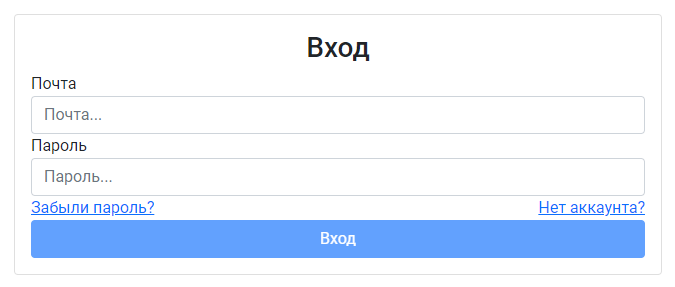
\includegraphics[scale=0.8]{attachments/register.png}  
	  \caption{ Форма входа в аккаунт после регистрации }
	  \label{sec:testing:func:register}
\end{figure}

\begin{table}[!htb]
	\caption{Тест-кейс аутентификации}
	\label{table:testing:func:test2}
	\centering
	  \begin{tabular}{| >{\raggedright}m{0.4\textwidth} 
					  | >{\raggedright}m{0.3\textwidth} 
					  | >{\raggedright\arraybackslash}m{0.2\textwidth}|}
	  \hline Тест & Ожидаемый результат  & Результат \\
	  \hline \textbf{Вход в аккаунт} \\ 1. Перейти во вкладку "Вход" на навигационной панели сайта \\ 2. Заполнить почту и пароль используя значения из предыдущего тест-кейса и нажать на кнопку "Вход" & 1. Появление формы для входа \\ 2. Перенаправление на страницу с каталогом игр & Успех (Рисунок \ref*{sec:testing:func:login})\\
	  \hline
	  \end{tabular}
\end{table}

\begin{figure}[!htb]
	\centering
	  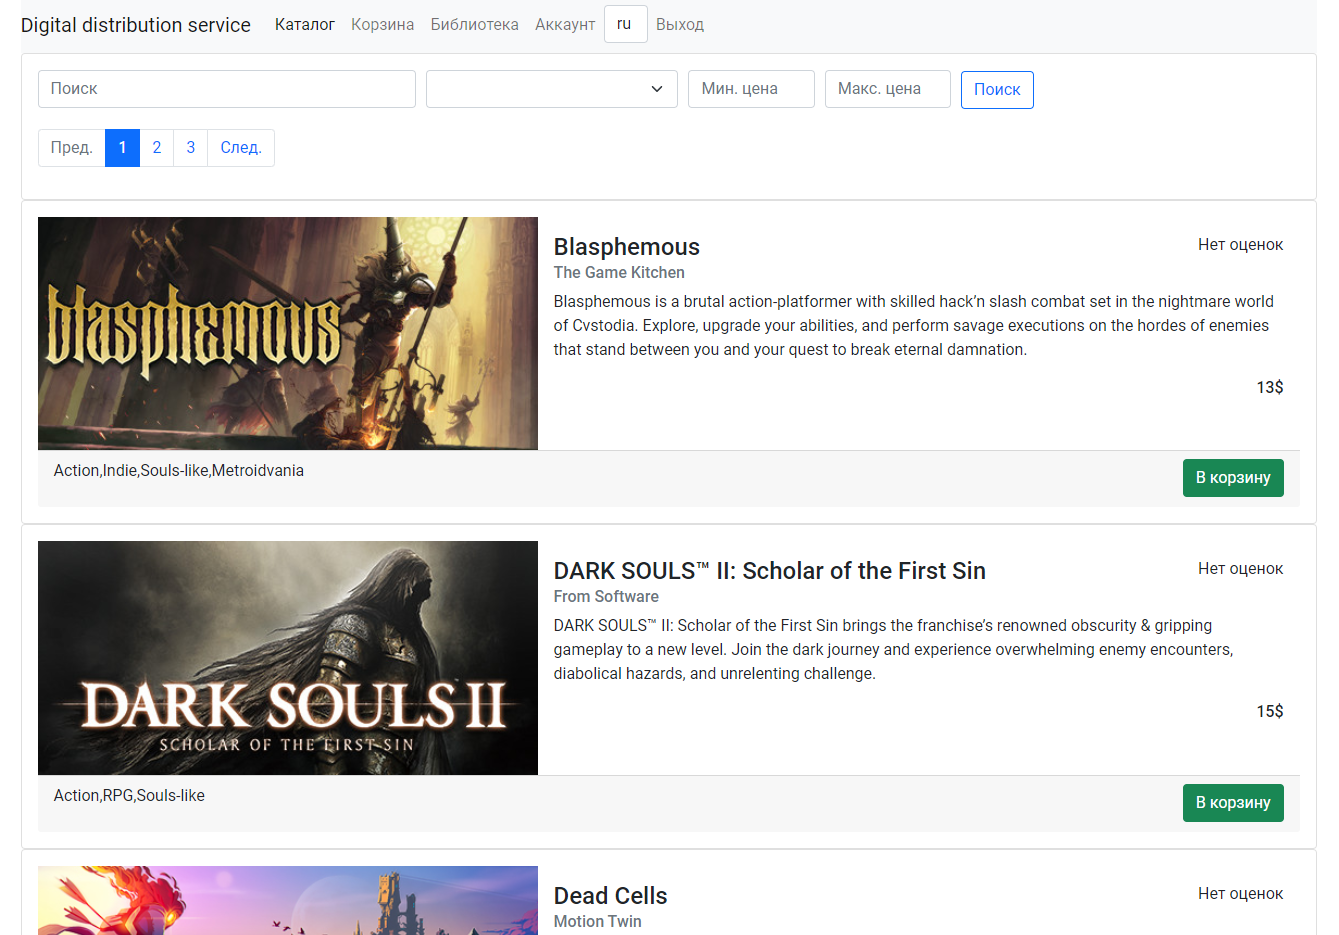
\includegraphics[scale=0.4]{attachments/login.png}  
	  \caption{ Страница с каталогом после успешного входа }
	  \label{sec:testing:func:login}
\end{figure}

\begin{table}[!htb]
	\caption{Тест-кейс восстановления доступа к аккаунту}
	\label{table:testing:func:test3}
	\centering
	  \begin{tabular}{| >{\raggedright}m{0.4\textwidth} 
					  | >{\raggedright}m{0.3\textwidth} 
					  | >{\raggedright\arraybackslash}m{0.2\textwidth}|}
	  \hline Тест & Ожидаемый результат  & Результат \\
	  \hline \textbf{Восстановление доступа к аккаунту} \\ 1. Перейти во вкладку "Вход" на навигационной панели сайта \\ 2. Нажать на кнопку "Забыли пароль?" \\ 3. Ввести почту и нажать на кнопку "Отправить" справа от поля \\ 4. Ввести полученный по почте код и нажать на кнопку "Отправит" внизу формы & 1. Появление формы для входа \\ 2. Появление формы для восстановления доступа \\ 3. Получения письма с кодом на указанный почтовый ящик \\ 4. Перенаправление на страницу смены пароля & Успех (Рисунки \ref*{sec:testing:func:mailmsg}, \ref*{sec:testing:func:passwordchange})\\
	  \hline
	  \end{tabular}
\end{table}

\begin{figure}[!htb]
	\centering
	  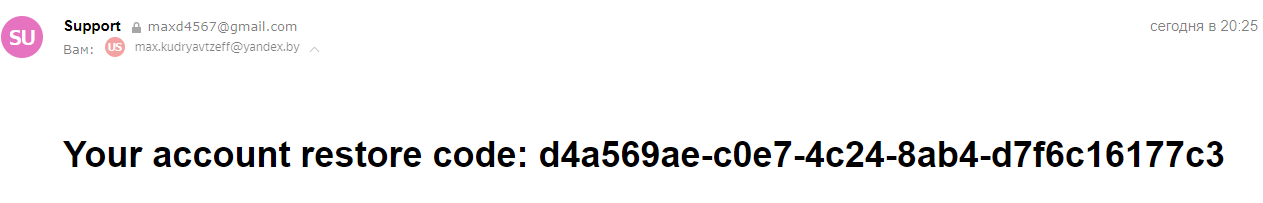
\includegraphics[scale=0.45]{attachments/mailmsg.png}  
	  \caption{ Письмо с кодом, полученное на указанный почтовый ящик }
	  \label{sec:testing:func:mailmsg}
\end{figure}
\clearpage
\begin{figure}[!ht]
	\centering
	  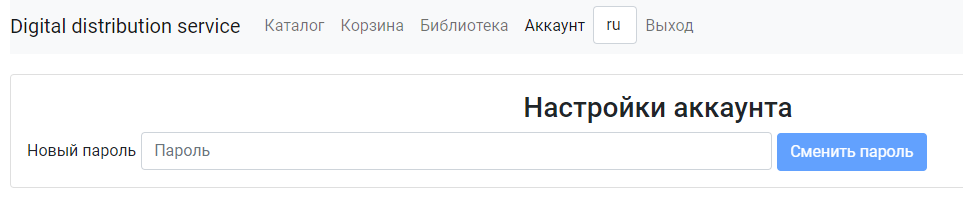
\includegraphics[scale=0.5]{attachments/passwordchange.png}  
	  \caption{ Форма для смены пароля }
	  \label{sec:testing:func:passwordchange}
\end{figure}

\begin{table}[h]
	\caption{Тест-кейс добавления игр в корзину}
	\label{table:testing:func:test4}
	\centering
	  \begin{tabular}{| >{\raggedright}m{0.4\textwidth} 
					  | >{\raggedright}m{0.3\textwidth} 
					  | >{\raggedright\arraybackslash}m{0.2\textwidth}|}
	  \hline Тест & Ожидаемый результат  & Результат \\
	  \hline \textbf{Добавление игр в корзину} \\ 1. Зайти в аккаунт \\ 2. Добавить несколько игр в корзину \\ 3. Перейти на страницу "Корзина" в навигационной панели & 1. Перенаправление на страницу "Каталог" \\ 2. Кнопки "В корзину" становятся неактивными \\ 3. В корзине отображаются добавленные игры & Успех (Рисунок \ref*{sec:testing:func:cart})\\
	  \hline
	  \end{tabular}
\end{table}

\begin{figure}[!h]
	\centering
	  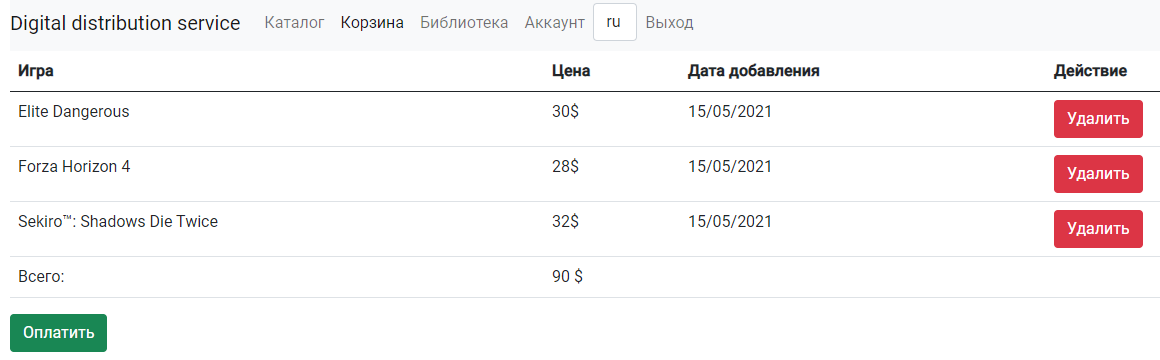
\includegraphics[scale=0.4]{attachments/cart.png}  
	  \caption{ Корзина пользователя }
	  \label{sec:testing:func:cart}
\end{figure}

\begin{table}[!htb]
	\caption{Тест-кейс приобретения игр}
	\label{table:testing:func:test5}
	\centering
	  \begin{tabular}{| >{\raggedright}m{0.4\textwidth} 
					  | >{\raggedright}m{0.3\textwidth} 
					  | >{\raggedright\arraybackslash}m{0.2\textwidth}|}
	  \hline Тест & Ожидаемый результат  & Результат \\
	  \hline \textbf{Приобретение игр} \\ 1. Зайти в аккаунт и перейти на страницу "Корзина" в навигационной панели \\ 2. Нажать на кнопку "Оплатить" & 1. Перенаправление на страницу "Корзина" со списком добавленных игр \\ 2. Перенаправление на страницу "Библиотека" с приобретёнными играми & Успех (Рисунок \ref*{sec:testing:func:library})\\
	  \hline
	  \end{tabular}
\end{table}
\clearpage
\begin{figure}[!ht]
	\centering
	  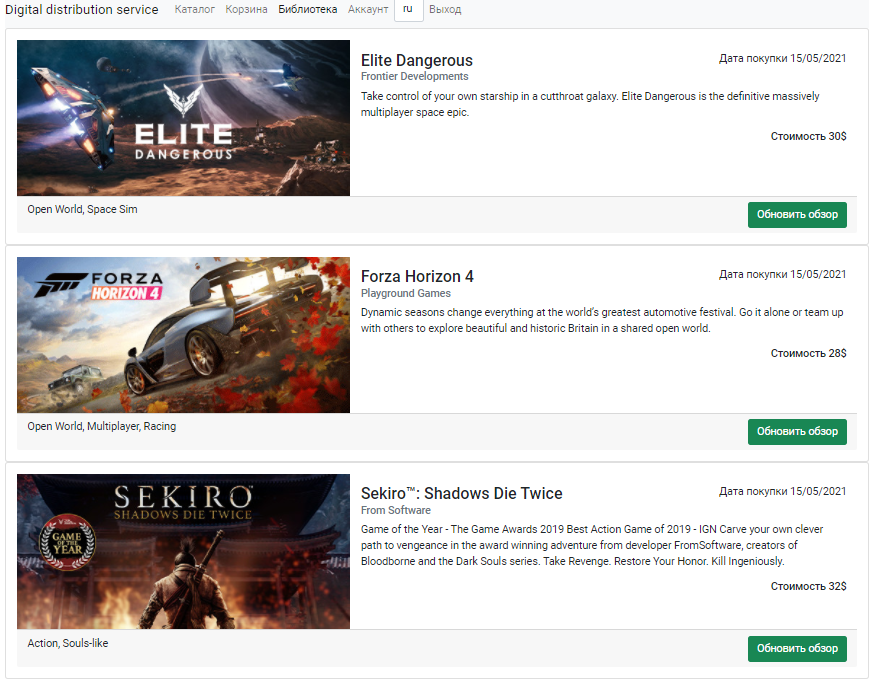
\includegraphics[scale=0.5]{attachments/library.png}  
	  \caption{ Библиотека пользователя }
	  \label{sec:testing:func:library}
\end{figure}

\begin{table}[!htb]
	\caption{Тест-кейс добавления отзыва}
	\label{table:testing:func:test6}
	\centering
	  \begin{tabular}{| >{\raggedright}m{0.4\textwidth} 
					  | >{\raggedright}m{0.3\textwidth} 
					  | >{\raggedright\arraybackslash}m{0.2\textwidth}|}
	  \hline Тест & Ожидаемый результат  & Результат \\
	  \hline \textbf{Добавление отзыва} \\ 1. Зайти в аккаунт и перейти на страницу "Библиотека" в навигационной панели \\ 2. Нажать на кнопку "Обновить обзор" напротив выбранной игры \\ 3. Заполнить поля и нажать кнопку "Обновить" \\ 4. Перейти на страницу "Каталог" & 1. Перенаправление на страницу "Библиотека" с приобретёнными играми \\ 2. Появление формы для отзыва \\ 3. Появление надписи "Success" \\ 4. Напротив игры отображается её оценка & Успех (Рисунок \ref*{sec:testing:func:review})\\
	  \hline
	  \end{tabular}
\end{table}

\begin{figure}[!htb]
	\centering
	  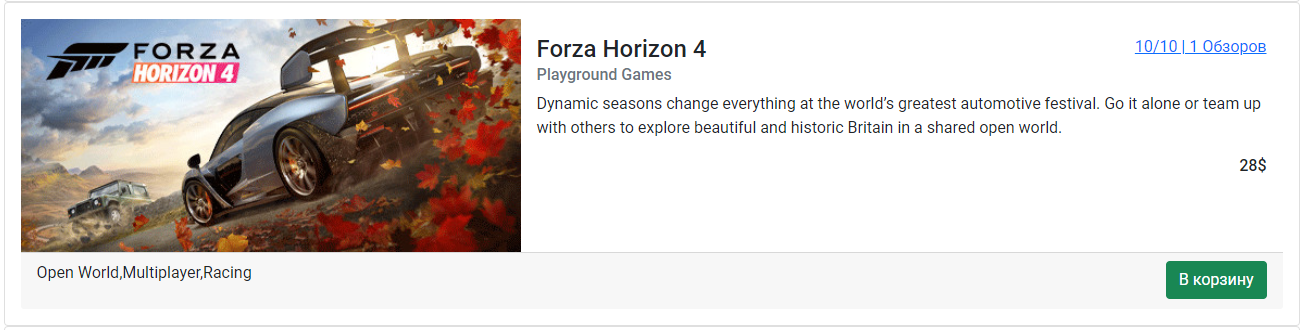
\includegraphics[scale=0.33]{attachments/review.png}  
	  \caption{ Игра с отзывами }
	  \label{sec:testing:func:review}
\end{figure}
\clearpage
\begin{table}[!ht]
	\caption{Тест-кейс смены локализации}
	\label{table:testing:func:test7}
	\centering
	  \begin{tabular}{| >{\raggedright}m{0.4\textwidth} 
					  | >{\raggedright}m{0.3\textwidth} 
					  | >{\raggedright\arraybackslash}m{0.2\textwidth}|}
	  \hline Тест & Ожидаемый результат  & Результат \\
	  \hline \textbf{Смена локализации} \\ 1. Зайти в аккаунт и перейти на страницу "Каталог" \\ 2. В навигационной панели выбрать английский язык & 1. Перенаправление на страницу "Каталог" \\ 2. Локализация сайта сменилась на английскую & Успех (Рисунок \ref*{sec:testing:func:en})\\
	  \hline
	  \end{tabular}
\end{table}

\begin{figure}[!htb]
	\centering
	  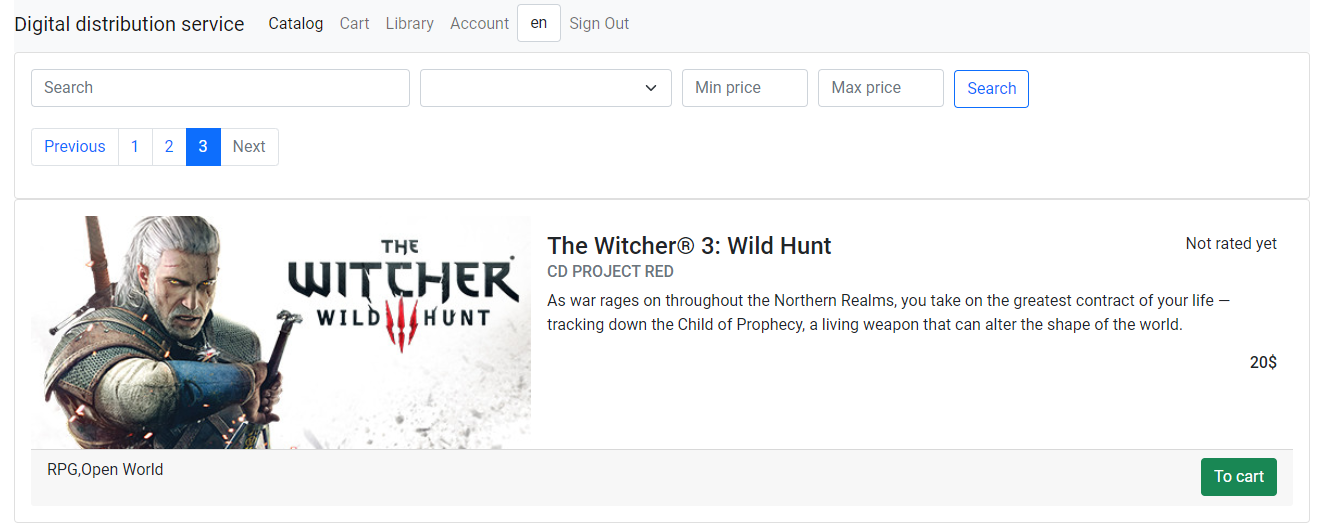
\includegraphics[scale=0.4]{attachments/en.png}  
	  \caption{ Ангийская локализация сайта }
	  \label{sec:testing:func:en}
\end{figure}

